\documentclass[]{beamer}

\usepackage{amssymb}
\usepackage{amsthm}

\newtheorem{proposition}{Proposition}

\usepackage{xcolor}
\usepackage{tikz}
\usetikzlibrary{shapes,arrows,calc}

\usepackage{tcolorbox}

\usepackage{minted}

\newcommand{\R}{{\mathbb R}}
\newcommand{\N}{{\mathbb N}}
\newcommand{\E}{{\mathbb E}}
\renewcommand{\P}{{\mathbb P}}

\newcommand{\cO}{\mathcal{O}}
\newcommand{\cF}{\mathcal{F}}
\newcommand{\cE}{\mathcal{E}}
\newcommand{\cX}{\mathcal{X}}
\newcommand{\cA}{\mathcal{A}}
\newcommand{\cS}{\mathcal{S}}
\newcommand{\cR}{\mathcal{R}}
\newcommand{\cB}{\mathcal{B}}

\newcommand{\tV}{\widetilde{V}}
\newcommand{\tF}{\widetilde{F}}
\newcommand{\tQ}{\widetilde{Q}}

\newcommand{\bw}{\mathbold{w}}

\newcommand{\step}[1]{\mathds{1}_{\{#1\ge 0\}}}

\newcommand{\eps}{\varepsilon}

\renewcommand{\emph}[1]{\textcolor{purple}{#1}}

\newcommand{\argmax}{\mathop{\textrm{argmax}}}
\newcommand{\mean}{\mathop{\textrm{mean}}}
\newcommand{\diam}{\mathop{\textrm{diam}}}


% presentation metadata
\title{GAIO}
\subtitle{25 years later}
\author{Oliver Junge}

\institute{Department of Mathematics\\Technical University of Munich}
\date{}


\setlength{\parskip}{1em}

\usepackage{mathpple}
%\usepackage{euler}
%\usepackage{palatino}

\begin{document}

\maketitle

\begin{frame}{Where it all started}

\begin{center}
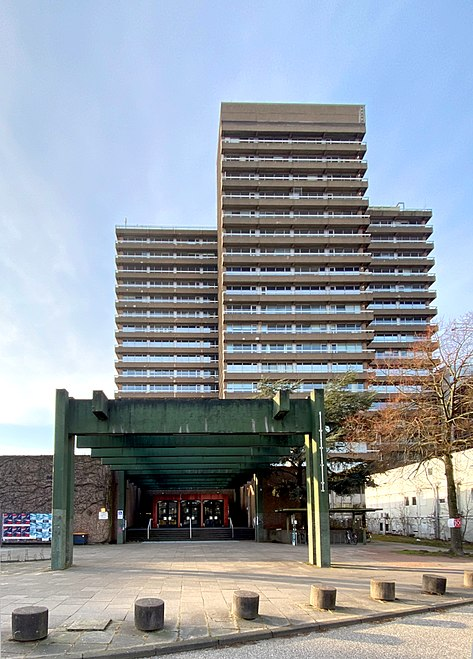
\includegraphics[height=0.8\textheight]{figures/geomatikum-1}
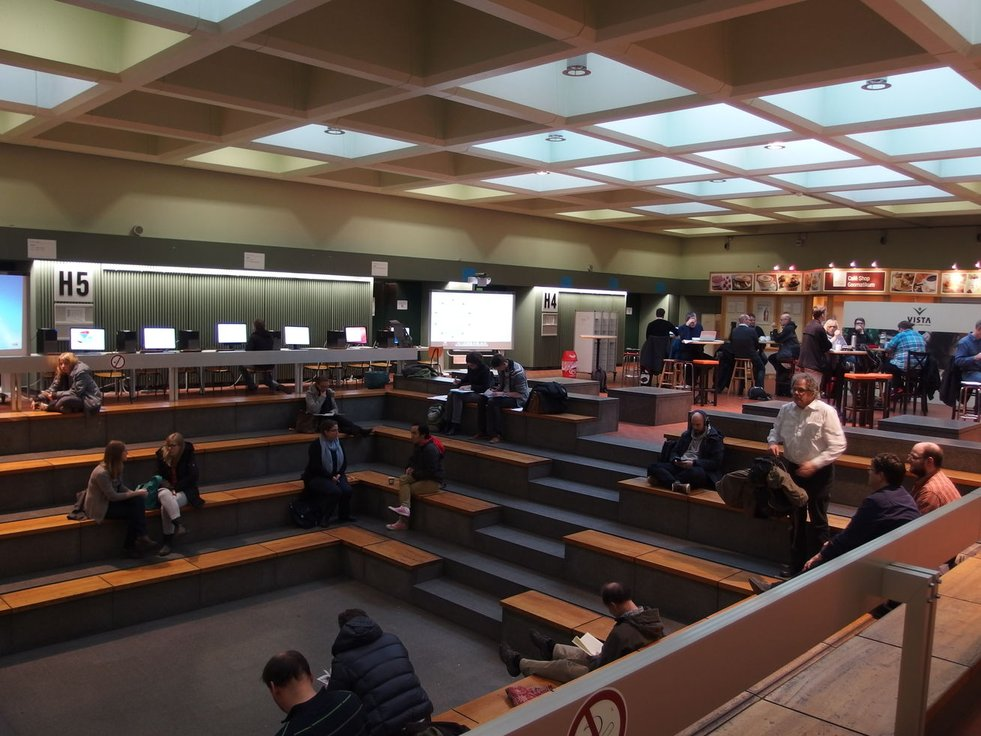
\includegraphics[height=0.8\textheight]{figures/geomatikum-2}
\end{center}

\end{frame}

\begin{frame}{Who it all started}

\begin{center}
    
\includegraphics[height=0.8\textheight]{figures/dellnitz-2011}
\end{center}

\end{frame}


\begin{frame}{With what it all started}

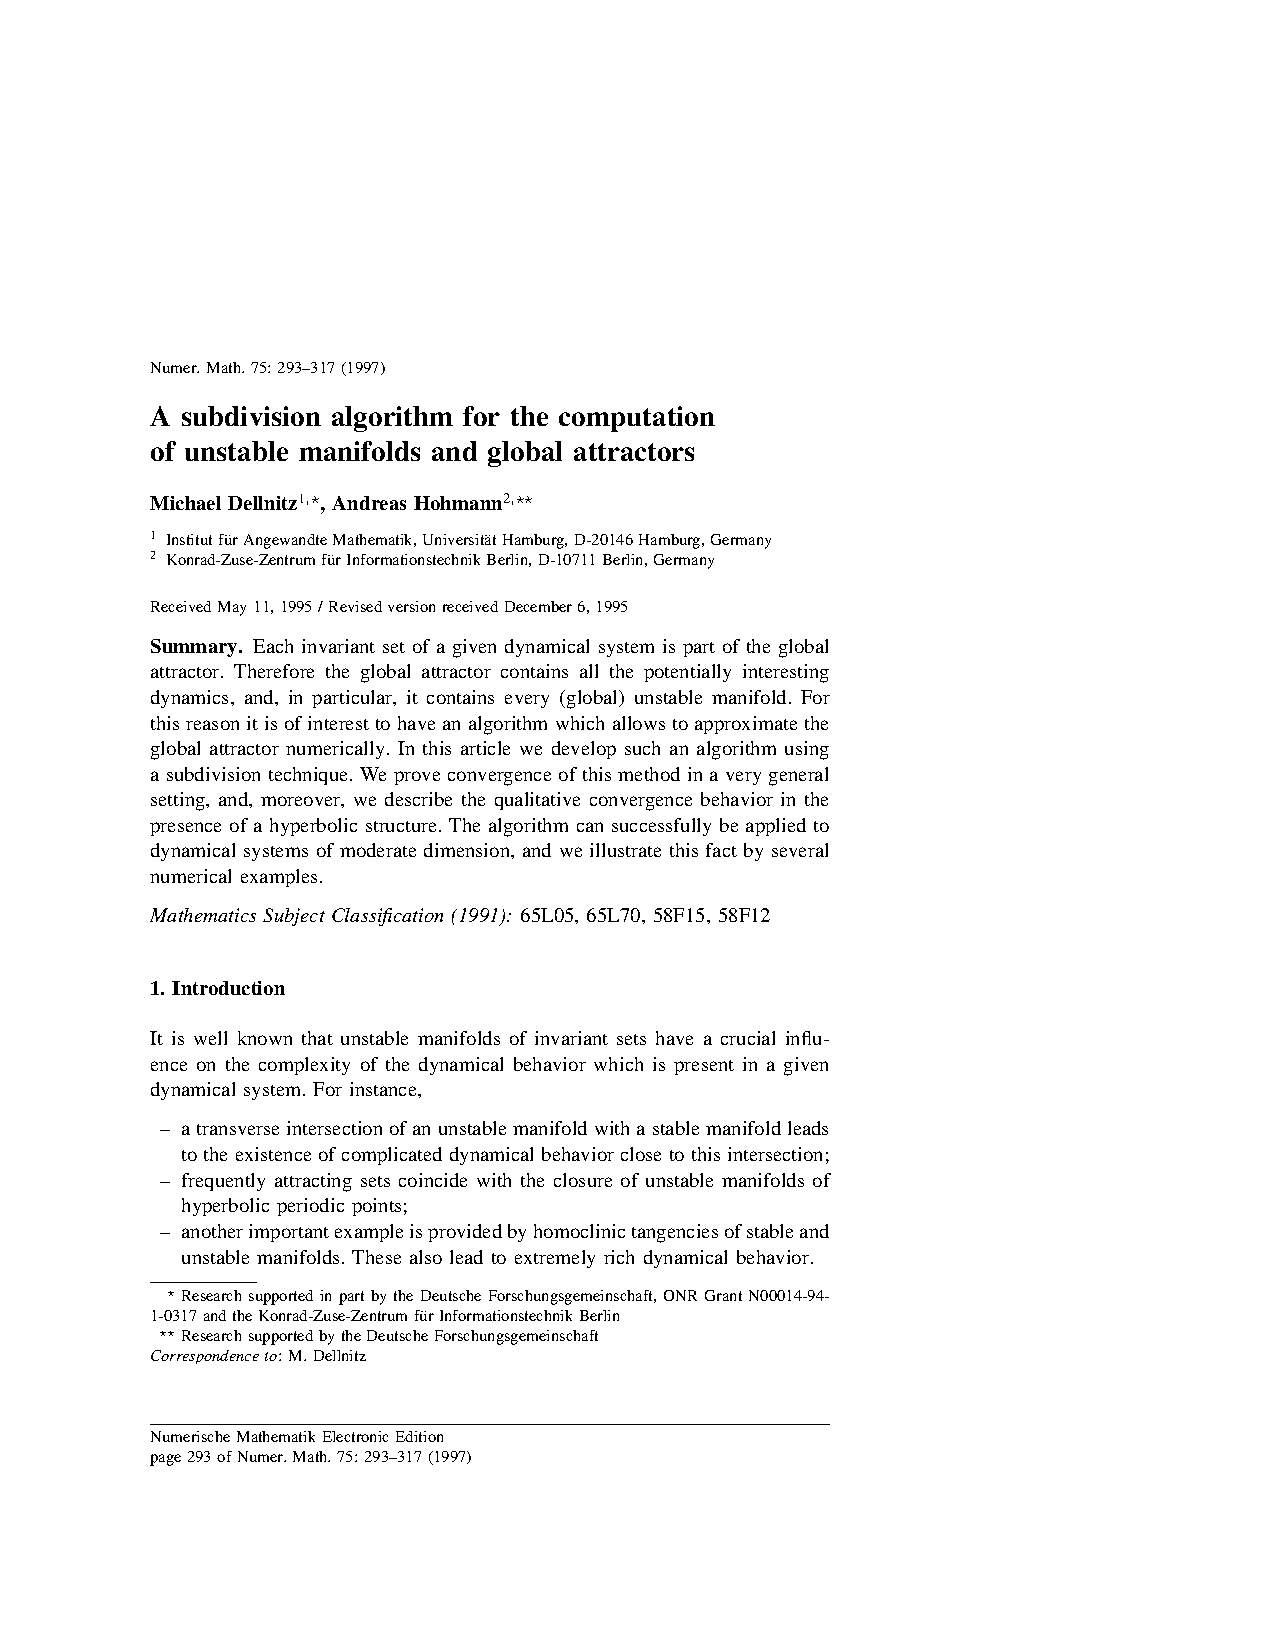
\includegraphics[trim=0 0 0 160,clip,width=1.3\textwidth]{figures/DH97}

\end{frame}

\begin{frame}{Dynamical systems}

Consider a continuous map
\[
f:\R^d\to \R^d.
\] 

The map defines a \emph{discrete dynamical system} by iteration:
\[
x_{k+1} = f(x_k), \qquad k=0,1,2,\ldots
\]

\begin{tcolorbox}[colback=blue!5!white,colframe=blue!75!black]
Basic question: \textit{What is the fate of some $x_0$ as $k\to\infty$?}
\end{tcolorbox}



\end{frame}

\begin{frame}{Attractors}

\begin{definition}
    A set $A\subset\R^d$ is \emph{invariant}, if
    \[
    f(A)=A.
    \]
\end{definition}

\begin{tcolorbox}[colback=blue!5!white,colframe=blue!75!black]
Example: $A=\{\bar x\}$ with $\bar x = f(\bar x)$ a \emph{fixed point}.
\end{tcolorbox}


\begin{definition}
    An invariant set $A$ is \emph{attracting} if there is a neighborhood $U$ of $A$ such that for every open set $V\supset A$ there is $K\in\N$ such that
    \[
    f^k(U)\subset V \quad\text{for all } k\ge K.
    \]
\end{definition}

\end{frame}

\begin{frame}{Relative attractors}

\begin{proposition}
    If $A$ is a closed invariant set then
    \[
    A = \bigcap_{k\in\N} f^k(U).
    \]
\end{proposition}

\begin{definition}
    For some compact set $Q\subset\R^d$, the \emph{attractor relative to} $Q$ is
    \[
    A_Q \overset{def}{=} \bigcap_{k\in\N} f^k(Q).
    \]    
\end{definition}

We have
\begin{itemize}
    \item $A_Q$ is not necessarily invariant,
    \item but any invariant subset of $Q$ is contained in $A_Q$.  
\end{itemize}

\end{frame}

\begin{frame}{Computing $A_Q$}

Generate a sequence $\cB_0,\cB_1,\cB_2,\ldots$ of finite families of compact sets as follows:

Let $\cB_0=\{Q\}$, $\theta \in (0,1)$. For $k=1,2,\ldots$ do
\begin{itemize}
    \item construct $\hat\cB_k$ such that
    \[
    |\hat\cB_k| = |\cB_{k-1}|
    \quad\text{and}\quad \diam\hat\cB_k \leq \theta \diam\cB_{k-1}.
    \]
    \item set
    \[
    \cB_k = \{ B\in\hat\cB_k \mid \exists B'\in\hat\cB_k: f^{-1}(B)\cap B' \neq \varnothing\}.
    \]
\end{itemize}

\medskip

\begin{theorem}
$|\cB_k|\to A_Q$ as $k\to\infty$ in the Hausdorff metric.
\end{theorem}

\end{frame}

\begin{frame}{Implementation}

Storage of the $\cB_k$ in a \emph{binary tree}, subdivision by bisection:


\end{frame}

\begin{frame}{GAIO v0.2}

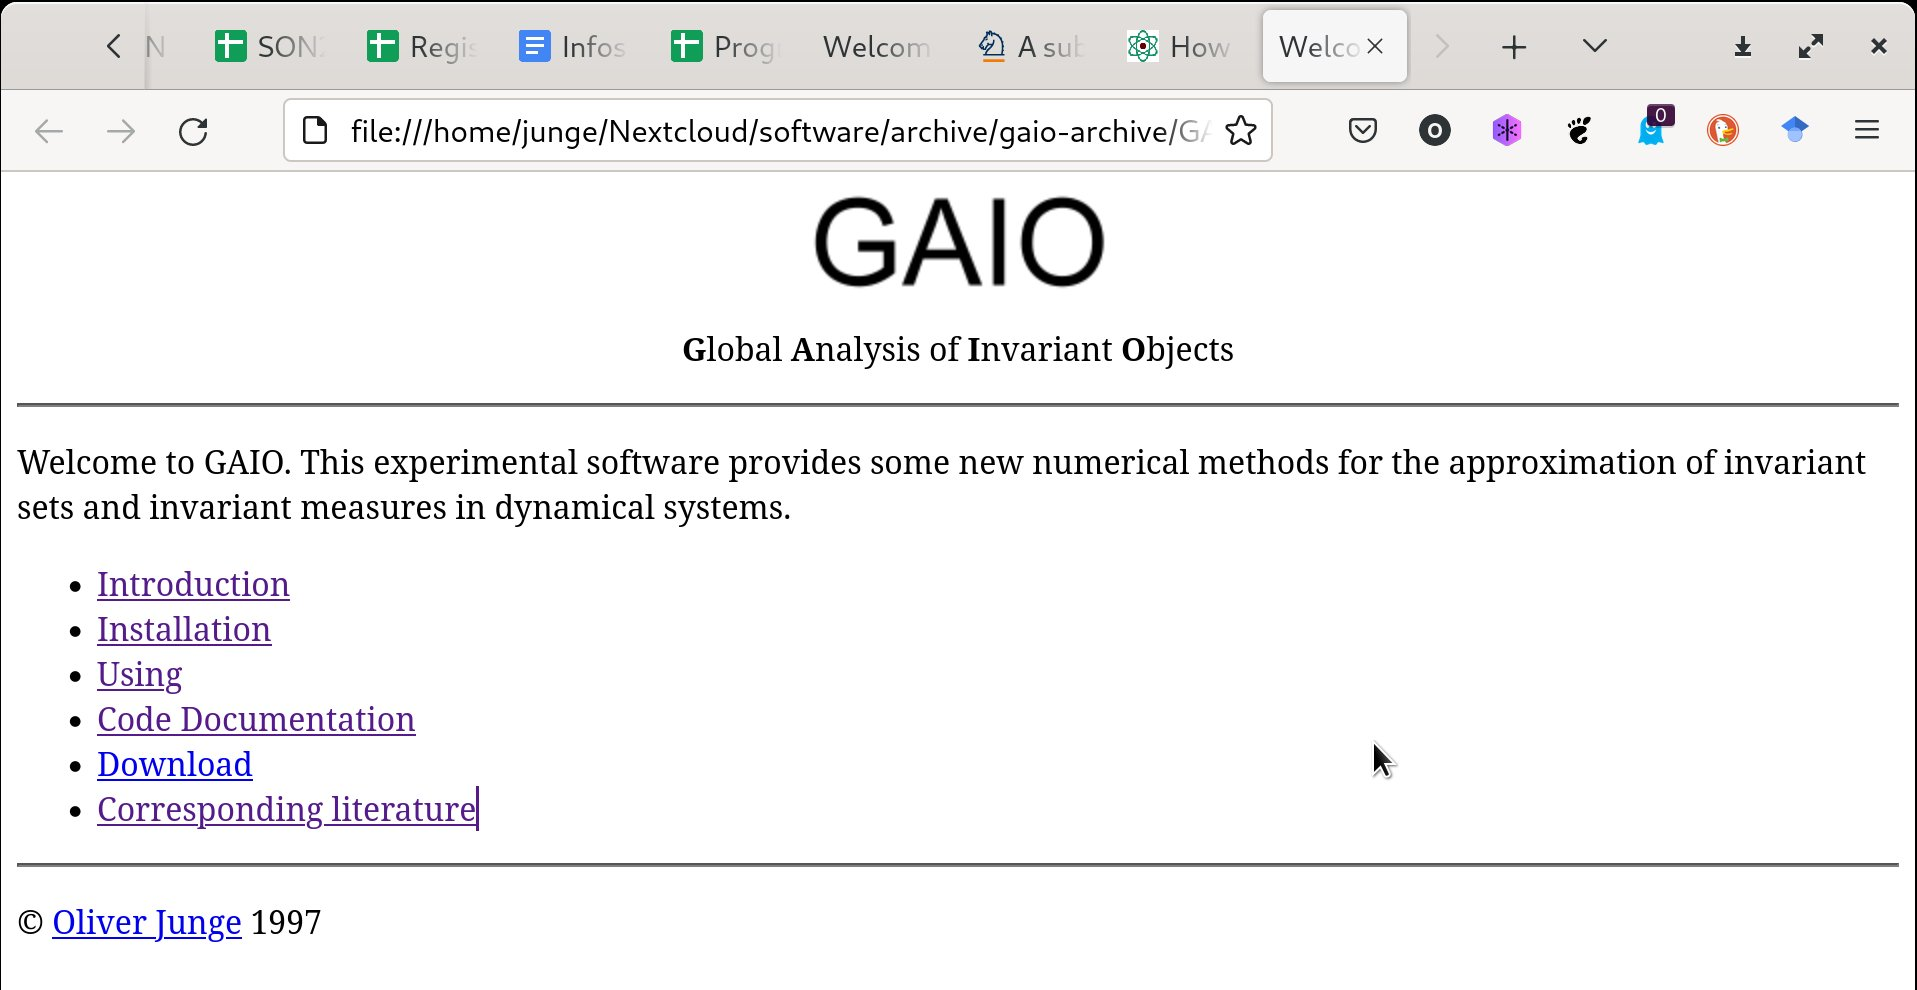
\includegraphics[trim=0 0 0 140,clip,width=\textwidth]{figures/GAIO_0.2}

\end{frame}

\begin{frame}{Architecture}





\end{frame}

\begin{frame}{Architecture}[fragile]

\begin{minted}
import numpy as np
    
def incmatrix(genl1,genl2):
    m = len(genl1)
    n = len(genl2)
    M = None to become the incidence matrix
    VT = np.zeros((n*m,1), int)  dummy variable
        
    return M
\end{minted}

\end{frame}

\end{document}
